\documentclass[tikz,border=8pt]{standalone}
\usepackage[T1]{fontenc}
\usepackage{lmodern}
\usepackage{amsmath}
\usetikzlibrary{arrows.meta,calc}

% Breadth-first (binary-heap) numbering: the children of v are 2v and 2v+1.
% These lists control both the tree symbols and the displayed configuration.
\newcommand{\PebbledVertices}{2,6,8,9,10,11,12,13,14,15}
\newcommand{\GhostVertices}{3,4}
\newcommand{\EmptyVertices}{1,5,7}

\definecolor{edgegray}{gray}{0.20}
\definecolor{pebblegray}{gray}{0.49}

% Each symbol is centered on its vertex. Labels are placed uniformly below it.
\newcommand{\pebblesymbol}[1]{%
  \begin{scope}[shift={#1}]
    \shade[shading=axis,top color=gray!20,bottom color=pebblegray,
      shading angle=25,draw=gray!65,line width=0.6pt]
      (-0.40,-0.06)
      .. controls (-0.43,0.10) and (-0.21,0.24) .. (0.07,0.23)
      .. controls (0.30,0.26) and (0.40,0.15) .. (0.41,-0.02)
      .. controls (0.43,-0.19) and (0.19,-0.25) .. (-0.09,-0.23)
      .. controls (-0.25,-0.22) and (-0.39,-0.17) .. cycle;
    \draw[white,opacity=0.65,line width=0.75pt,line cap=round]
      (-0.24,0.10) .. controls (-0.13,0.17) and (-0.02,0.18) .. (0.10,0.17);
  \end{scope}%
}

\newcommand{\ghostsymbol}[1]{%
  \begin{scope}[shift={#1}]
    \draw[edgegray,line width=0.8pt,dash pattern=on 2pt off 1.8pt,
      fill=white] (0,-0.08) ellipse[x radius=0.44,y radius=0.23];
    \draw[edgegray,fill=white,line width=0.85pt,
      line join=round,line cap=round]
      (-0.25,-0.15)
      .. controls (-0.22,-0.03) and (-0.22,0.08) .. (-0.22,0.17)
      .. controls (-0.22,0.33) and (-0.12,0.39) .. (0,0.39)
      .. controls (0.12,0.39) and (0.22,0.33) .. (0.22,0.17)
      .. controls (0.22,0.08) and (0.22,-0.03) .. (0.25,-0.15)
      .. controls (0.20,-0.10) and (0.16,-0.22) .. (0.10,-0.16)
      .. controls (0.06,-0.12) and (0.02,-0.22) .. (-0.03,-0.17)
      .. controls (-0.08,-0.12) and (-0.12,-0.23) .. (-0.17,-0.17)
      .. controls (-0.21,-0.13) and (-0.23,-0.18) .. cycle;
    \draw[edgegray,fill=white,line width=0.6pt]
      (-0.075,0.20) ellipse[x radius=0.034,y radius=0.050];
    \draw[edgegray,fill=white,line width=0.6pt]
      (0.075,0.20) ellipse[x radius=0.034,y radius=0.050];
    \draw[edgegray,line width=0.65pt,line cap=round]
      (-0.044,0.085) .. controls (0,0.035) and (0.025,0.055) .. (0.047,0.095);
  \end{scope}%
}

\newcommand{\emptysymbol}[1]{%
  \draw[edgegray,line width=0.85pt,dash pattern=on 2pt off 1.8pt,
    fill=white] #1 ellipse[x radius=0.44,y radius=0.23];
}

\begin{document}
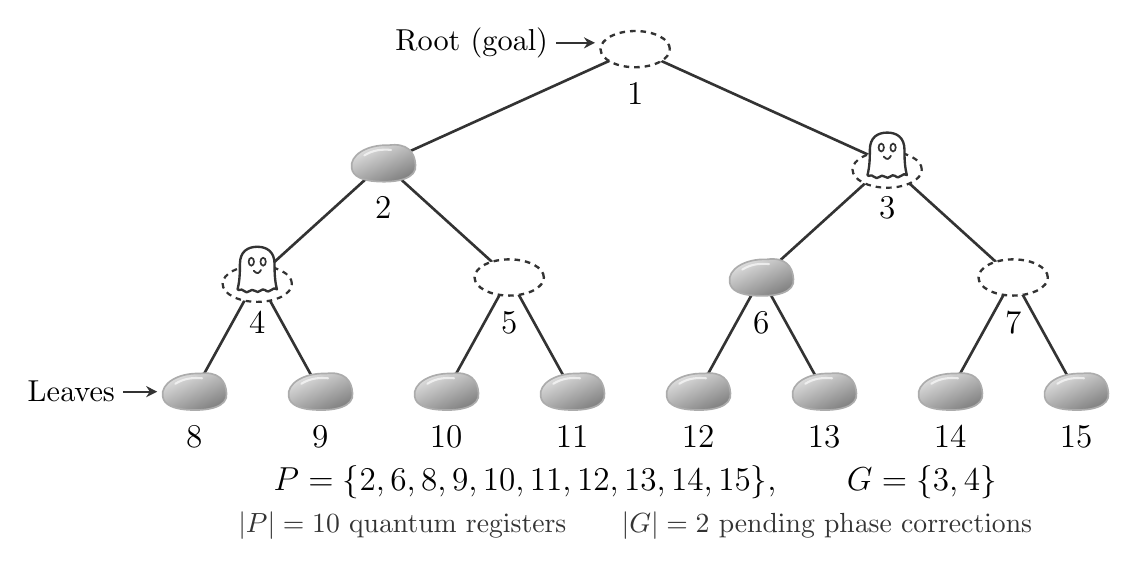
\begin{tikzpicture}[
  x=1cm,y=1cm,
  edge/.style={draw=edgegray,line width=0.95pt},
  vertex label/.style={font=\fontsize{12}{14}\selectfont,inner sep=0pt},
  callout/.style={font=\fontsize{11}{13}\selectfont,inner sep=0pt}
]
  % A symmetric layout, with equal spacing at each vertex level.
  \foreach \v in {1,...,15} {
    \pgfmathtruncatemacro{\level}{floor(ln(\v)/ln(2)+0.00001)}
    \pgfmathsetmacro{\xx}{(\v-pow(2,\level)+0.5)*12.8/pow(2,\level)-6.4}
    \pgfmathsetmacro{\yy}{-1.45*\level}
    \coordinate (v\v) at (\xx,\yy);
  }

  % Draw dependencies first, so all vertex symbols mask their endpoints.
  \foreach \v in {2,...,15} {
    \pgfmathtruncatemacro{\parent}{floor(\v/2)}
    \draw[edge] (v\parent) -- (v\v);
  }

  \foreach \v in \EmptyVertices {\emptysymbol{(v\v)}}
  \foreach \v in \PebbledVertices {\pebblesymbol{(v\v)}}
  \foreach \v in \GhostVertices {\ghostsymbol{(v\v)}}

  \foreach \v in {1,...,15} {
    \node[vertex label] at ($(v\v)+(0,-0.57)$) {$\v$};
  }

  \node[callout,anchor=east] (goal) at (-1.10,0.08) {Root (goal)};
  \draw[edgegray,line width=0.8pt,-{Stealth[length=4pt,width=4pt]}]
    (-1.00,0.08) -- (-0.51,0.08);

  \node[callout,anchor=east] (leaves) at (-6.60,-4.35) {Leaves};
  \draw[edgegray,line width=0.8pt,-{Stealth[length=4pt,width=4pt]}]
    (-6.50,-4.35) -- (-6.07,-4.35);

  % The displayed snapshot has ten stored values and two pending corrections.
  \node[font=\fontsize{12}{15}\selectfont,inner sep=0pt] at (0,-5.50)
    {$P=\{\PebbledVertices\},\qquad G=\{\GhostVertices\}$};
  \node[font=\fontsize{10}{12}\selectfont,inner sep=0pt,text=edgegray]
    at (0,-6.05)
    {$|P|=10$ quantum registers\qquad $|G|=2$ pending phase corrections};
\end{tikzpicture}
\end{document}
